\chapter{Introduction}
Analysis of electrical machines is a very well-known subject in electrical engineering and at a first glance one might think that this field cannot be embarked on any further. However, this is not the case, since advances in materials such as permanent magnets offer new possibilities which might not have been economical a few years ago. In addition to the development of the materials used in electrical machines, the mathematical and physics software tools for solving complex problems and the visualisation of the results have also improved. Furthermore, the technologies driving the microprocessors and storage devices used in personal computers have contributed to solve difficult mathematical functions by means of numerical methods. All these factors have influenced the way electrical machines are designed and will be designed in the future. The research presented in this dissertation is a typical example of how advances in other fields can lead to new ideas in electrical engineering, and especially electrical machines. 


\section{Background to the study}
At present most of all existing variable speed drive systems are still based on induction machines. A typical example are traction drives for rail vehicles. Today, the state of the art drive system of metro trains with underfloor traction equipment consists of a 3-phase IGBT converter feeding two or four induction traction machines in parallel. For the torque transmission to the wheel-set a gearbox is needed, because the induction machine cannot develop sufficient torque in the available space. For the transport operator the gearbox means investment, maintenance, undesired noise and losses. Furthermore, \cite{Joeckel2006} mentioned that the very high torque developed during a terminal short circuit, which arises from an inverter failure, leads to over-sized mechanical components. In order to reduce energy loss, investment and maintenance costs there is a trend to replace the induction motor and gearbox with a direct drive system as pointed out by \cite{joeckel_2006_EB}. This not only improves efficiency and performance, but also the life cycle costs, as shown by \cite{germishuizen_2006}.  

The machine that is used in a direct drive system  requires a high torque to weight ratio, high efficiency and a wide speed range for constant power. The permanent magnet synchronous machine fulfills these requirements. \cite{gieras_2000} compared different machine types and showed that the permanent magnet synchronous machine has the highest torque density and highest efficiency. The machine can also be used for different applications ranging from low speed to high speed. Compared to the induction machine the permanent magnet synchronous machine can be designed with a greater variety of winding layouts. These advantages make it therefore feasible to design direct drive traction machines using permanent magnet technology. Usually such designs lead to a machine with a high pole number and often with a fractional slot winding.

\cite{koch_2001} investigated the performance of permanent magnet machines for high speed trains. The suggested machine has a double layer winding comprising form-wound coils. This winding type has a high copper fill factor and although it was found that this winding type has a good performance it is still quite expensive due to the high number of form-wound coils. An alternative winding type is a non-overlapping single layer concentrated winding. Here only every second stator tooth has a coil wound around it. Advantages are the shorter end-winding overhang, the simplified winding insulation and a reduced number of stator coils as pointed out by \cite{cros_2002} as well as \cite{huth_2004}. The shorter overhang means that the active length can be increased. As a result the amount of copper in the end-windings is reduced. These advantages improve the efficiency and lead to reduced manufacturing costs. Drawbacks are the lower power factor and possible rotor heating due to the harmonic content of the air gap magnetomotive force (mmf). In general the higher harmonics in the air gap (and as a result the increased leakage inductance) cause higher core losses as reported by \cite{IR-EE-EME_2003:029}.

The design of the winding used in an electrical machine is often underestimated. This does not necessarily need to be seen as negative, since typically a manufacturer of machines will use approved designs. Such a policy has a lot to commend it. Resorting to approved designs means saving development costs and even a reduced design phase. With new materials available, older ideas which seem to be forgotten, can be investigated. Only then the real complexity of designing windings comes to the fore. 

The idea to replace the induction motor and gearbox with a direct drive is certainly not new. However, it was only until recently that the progress in material science made it possible to economically implement such a concept. On 12 August 2008 the Munich public transport company MVG started the operation of an underground train that is equipped with direct drive technology as reported by \cite{Tibudd2008}. It is the first of its kind and is a practical example of an innovative strategy and approach to integrate traction, bogie and braking technology. This new motor bogie technology weighs \SI{30}{\%} less than conventional state of the art motor bogies. The expected reduction in energy loss is estimated to be \SI{20}{\%} less than the present system in operation and will be tested over a period of two years.  

Due to the increasing demand to reduce manufacturing cost and weight, machine designs tend to become more compact. This leads to an increase in the torque per volume ratio. As a result, new materials with high magnetic energy density such as Neodymium-Iron-Boron (NdFeB) allow a very compact design in which case particularly the permanent magnet synchronous machine benefits. In addition, the emphasis on accurate performance estimations becomes essential and requires in many cases the use of numerical methods such as the finite element method. Compact designs also mean that the laminated parts are highly saturated and as a consequence the approximation of the material behaviour becomes an essential design component. And because of the lack of accuracy analytical solutions may lead to inadequate designs. Moreover, reducing costs may be achieved by the use of simple components which allow easy manufacturing. Therefore, a machine manufacturer has to keep track with all these aspects in order to be competitive.

\section{Problem statement}
\label{sec:problem_statement}
Designing the winding is from an electromagnetic point of view the most important part in machine design. In this step the coil sides of the phases need to be assigned to an appropriate stator slot which allows a rotating magnetic field when phase displaced currents are applied to the winding. Once the assignment is done, adjacent coil sides belonging to the same phase are called a phase belt. This is the definition used in modern textbooks such as that written by \cite{Fitzgerald1992} and was already in use in early papers by \cite{Kauders1932}\footnote{See \ref{sec:excursion} for a short portrait of Wilhelm Kauders.}.

When designing interior permanent magnet machines with non-overlapping concentrated windings it is necessary to have an inexpensive method which accurately calculates the machine's performance over a wide speed range. In addition, it is desirable to use the finite element method (FEM) since it takes into account the actual machine geometry as well as the non-linear material properties. Additionally, it should be fast and suitable in an everyday design environment. Therefore the main research question of the present dissertation is: 
\begin{quote}
\textbf{How can an analysis method be described to accurately calculate the performance of interior permanent magnet motors with non-overlapping windings in an everyday design environment?}
\end{quote}

In order to answer the main research question, it is necessary to have a systematic algorithm to allocate the slots. Then, after doing this, the concentrated coils can be inserted in the appropriate slots. The immediate and essential sub-question that first needs to be answered is: 
\begin{quote}
\textbf{What is the mathematical expression to allocate the stator slots belonging to a phase belt?} 
\end{quote}

Another sub-question arises from the requirement to allocate the slots that belong to a phase belt. Especially when using FEM to analyse machines, the entering of the winding arrangement is a complex process. The problem is exacerbated if different winding types are to be analysed. Furthermore, in the conceptual design phase a compact representation of the winding could simplify the choice of the initial geometrical parameters. Therefore the second sub-question is: 
\begin{quote}
\textbf{How can a winding layout be represented in a compact form?} 
\end{quote}
 
\section{Overlapping and non-overlapping windings}\label{sec:def_con}  
Fig.~\ref{fig:flux_coils}(a) shows a double layer overlapping winding. In the drawing some of the coils are removed which makes it easier to identify the two layers. In (b) a non-overlapping single layer winding is shown. Only each second stator tooth has a coil wound around it. 
\begin{figure}[htbp]
	\centering
		\begin{psfrags}%
\psfragscanon

% text strings:
\psfrag{t01}{double layer coil}
\psfrag{t02}{single layer coil}
\psfrag{t03}[bc]{(a) Overlapping winding}
\psfrag{t04}[bc]{(b) Non-overlapping winding}
\psfrag{t05}[bc]{Stator tooth}

% Figure:
\includegraphics[width=1.00\textwidth]{figs/f_coils.eps}
\end{psfrags}%
	\caption{Double layer overlapping and single layer non-overlapping windings}
	\label{fig:flux_coils}
\end{figure}

Non-overlapping windings are a sub-set of fractional slot windings and need some extra discussion. It is often categorised as concentrated. This is not necessarily wrong but is incongruent with the formal definition. The opposite of a concentrated winding is a distributed winding. In the latter case a the coils of a given phase are distributed in several slots. When referring to overlapping and non-overlapping windings a concentrated winding could be defined as follows:
\begin{enumerate}
	\item Formally a concentrated winding is one where the number of slots per pole and~%
	phase equals one. In this case the coil pitch equals the pole pitch and it is~%
	categorised as overlapping. This means that each coil side of the winding is~%
	placed in a single slot. If the coil spans a pole pitch, it is called a full-pitch~%
	concentrated winding.
	\item Non-overlapping could also be classified as concentrated, but then it is not~%
	done in terms of the formal definition. Concentrated in this case means that a coil~%
	is concentrated around a stator tooth as shown in Fig.~\ref{fig:flux_coils}(b).
\end{enumerate}

A simplified illustration of single and double layer non-overlapping windings\footnote{In German these winding types are commonly referred to as ``Zahnspulen'' which means ``tooth coils''. Although tooth coils seem to be a very descriptive name for these windings, it is often called ``concentrated coils'' in the literature.} is shown in Fig.~\ref{fig:concen_coils} and the difference between them is given in Tab.~\ref{tab:single_vs_double}. For the purposes of the present dissertation a double layer winding is defined as follows:
\begin{defth}
  A double layer winding has two coil sides per stator slot. ``Double layer'' in the~%
  case of overlapping windings means that the coil sides in a slot are placed~% 
  radially in two layers. In the case of non-overlapping windings a~%
  ``double layer'' winding has two coil sides side by side.
\end{defth} 
\begin{table}[htbp]
  \caption{Difference between single and double layer windings}
  \label{tab:single_vs_double}
  \begin{tabularx}{\textwidth}{XX}
    \toprule
    \textbf{Single layer}  & \textbf{Double layer} \\\toprule
    In the case of the single layer winding each stator slot has only one coil side
    assigned to it as shown in Fig.~\ref{fig:concen_coils}(a).
    & 
    A double layer winding has two coil sides assigned to a stator slot as shown in
    Fig.~\ref{fig:concen_coils}(b).\\
    \bottomrule
  \end{tabularx}
\end{table}
\begin{figure}[htbp]
	\centering
		\begin{psfrags}%
\psfragscanon

% text strings:
\psfrag{t01}[bc]{(a) Single layer}
\psfrag{t02}[bc]{(b) Double layer}
\psfrag{t03}[bc]{$x \tau_s$}
\psfrag{t04}[bc]{$2\tau_s$}
\psfrag{t05}[bc]{$\tau_s$}

% Figure:
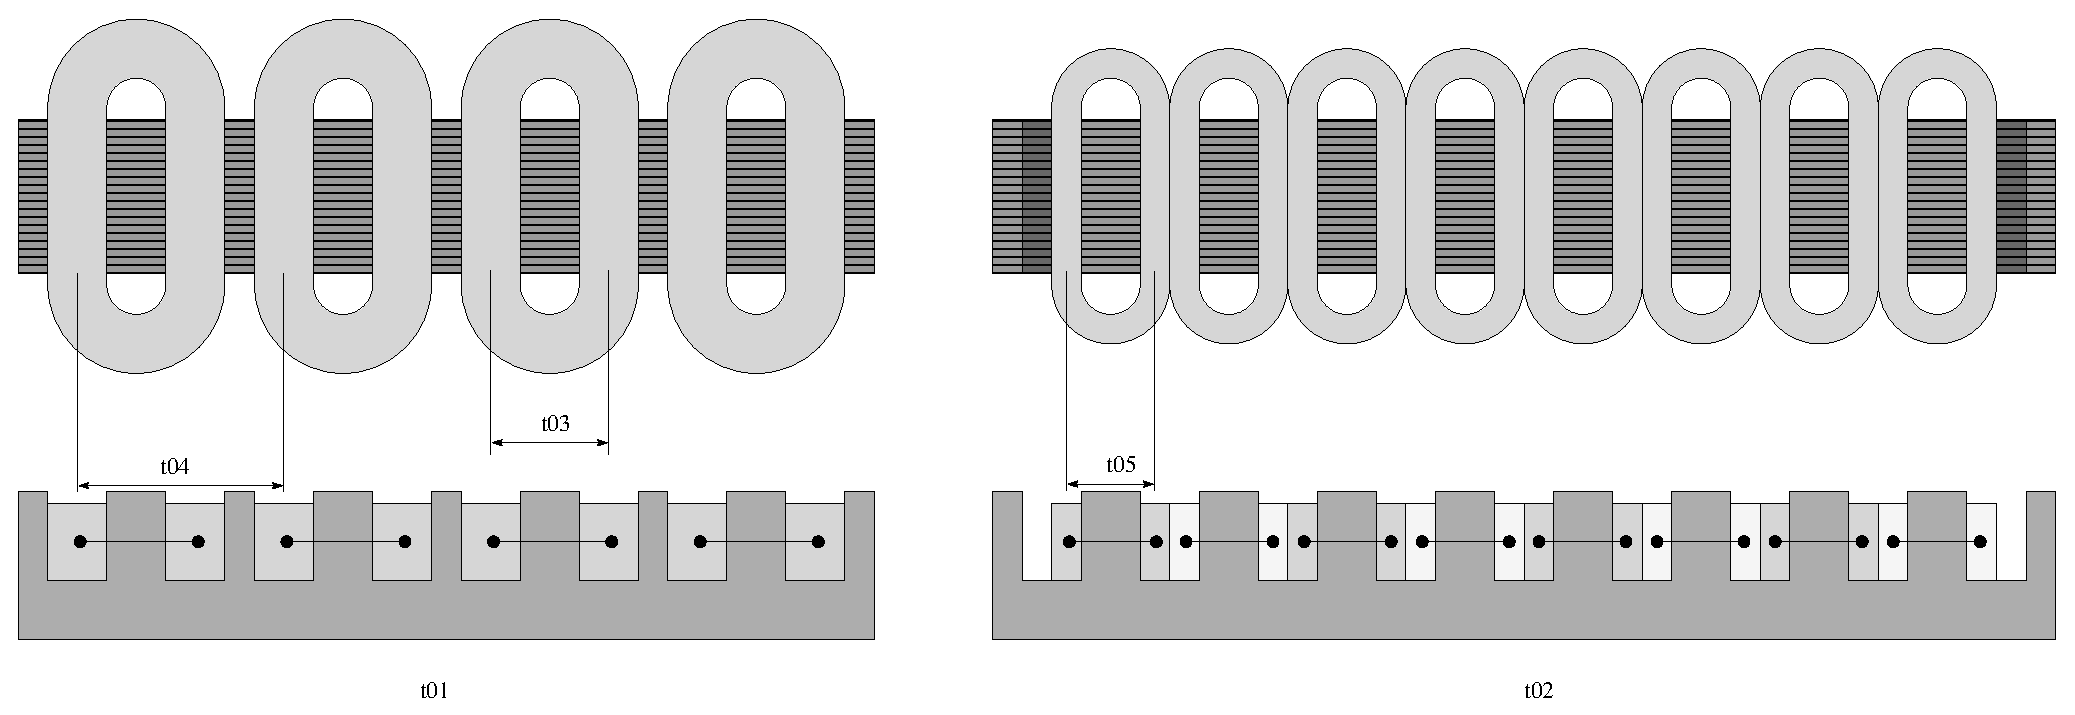
\includegraphics[width=1.00\textwidth]{figs/f_concen_coils.eps}
\end{psfrags}%
	\caption{Double and single layer non-overlapping windings}
	\label{fig:concen_coils}
\end{figure}

In the literature different definitions of terms are in use for non-overlapping concentrated windings. The most common of them are:
\begin{itemize*}
	\item \cite{IR-EE-EME_2003:029}: concentrated windings;
	\item \cite{IR-EE-EME_2004:022}: concentrated fractional pitch windings; 
	\item \cite{salminen_2004_ICEM}: fractional slot wound; and
	\item \cite{bianchi_2004}: fractional slot. 
\end{itemize*}

If the coils are to be equally in shape, which simplifies manufacturing, it is recognised that a single layer could easily have a variable slot pitch\footnote{The concept of a variable coil pitch is explained in chapter \ref{chap:DesignWindings}. Also refer to Fig.~\ref{fig:f_slotstar} for regular and irregular distributed slots.}. Furthermore, the coils could be implemented as either form-wound or round-wound. Returning to the variable coil pitch of the single layer, it is important to mention that this is an extra degree of freedom that offers to be an attractive design parameter. The air gap flux that links the coil could thus be increased and torque ripple can be improved. 

It is therefore helpful to classify a concentrated winding either as an overlapping or non-overlapping concentrated winding. \cite{cros_2002} certainly aroused interest in non-overlapping concentrated windings with their paper entitled ``Synthesis of High Performance PM Motors With Concentrated Windings'', since this is a paper which is very often used as a reference on these winding types. This could be a possible explanation for the use of the term ``concentrated windings'' rather than ``tooth coil windings''.

The expansion of the classical winding types used in machines by non-overlapping windings offers new possibilities in especially traction machine design. The main research question in section \ref{sec:problem_statement} suggests a design algorithm that takes into account the non-overlapping type. Obviously a method that is valid for all types is required. In addition, it should be easy to integrate into whichever process is in use. 

\section{Approach to the problem}
As a first step towards the analysis of interior permanent magnet synchronous machines with non-overlapping concentrated windings, an in depth overview of the systematics of $m$-phase windings is required. The paper of \cite{Kauders1932} and the book of \cite{Nuernerg1952} are two very good examples\footnote{This literature is unfortunately written in German, which means that it is not easily accessible for those with little or no German knowledge.}. A historical overview of winding design and tendencies in machine analyses are given in chapter \ref{chap:overview}.  

Addressing the research questions in section \ref{sec:problem_statement}, a good starting point would be to derive the air gap mmf using the classical single coil approach and then expand it for three phases. It would be ideal to find a systematic algorithm for assigning the coils to the stator slots. The derivation of the air gap mmf and winding theory is presented in chapter \ref{chap:DesignWindings}.

The new perspective on the winding representation and its properties offered in the present dissertation are then applied to a traction machine case study. Here only the degree of freedom that single layer non-overlapping windings provide, is focused on. This is explained in chapter \ref{chap:design}. Some important remarks on non-linear machine analysis to support the design results are explained in chapter \ref{chap:NonlinearAnalysis}.

A prototype and its measured results to verify the design process are given in section \ref{sec:prototype}. Finally, the conclusions and recommendations for further studies are presented in chapter \ref{chap:ConlusionsRecommendations}. 


\section{Scientific contributions of this dissertation}
The design of permanent magnet motors often results in the use of a fractional slot winding. Different methods are available to design these windings (which are often graphically presented), of which none takes into account single layer non-overlapping windings (which could have a variable slot pitch). Moreover, due to the different slot configurations, material non-linearities and saturation effects, it is impossible to find analytical methods to fulfill these requirements. In an everyday design environment it is necessary to have accurate and reliable tools. The scientific contribution of this dissertation can be summarised as follows:
\begin{itemize}
	\item A general method to design single layer non-overlapping windings with a 
	fixed and variable slot pitch is offered. The winding design is presented 
	in its most compact form and has all the information on the physical layout as 
	well as the winding harmonics. It will be shown that the developed method applies
	to $m$-phase windings in general as well.
	\item Developing an analytical model for the magnetic circuit of interior 
	permanent magnet motors is nearly impossible. A better method is to make use of 
	both the analytical and finite element method. The machine is characterised by 
	three (finite element analysis generated) two-dimensional functions and frequency
	dependent losses are calculated analytically.
	\item The methodology from the study is applied to a \SI{150}{kW} prototype motor 
	designed for a traction application. The manufactured machine has \num{30} stator
	slots and \num{20} poles. Practical measurements were done to verify the computational
	results presented.   
\end{itemize}	

\section{Delimitations of the study}
The aim of this study is the analysis of interior permanent magnet synchronous machines with single layer non-overlapping windings. A comparison with other machine types is not given. The single layer non-overlapping winding offers an inherent degree of freedom, namely the variable coil pitch. Since this is not typical for other\footnote{When referring to other winding types, it means double layer non-overlapping as well as single and double layer overlapping windings.} winding types, this will be the only design aspect that will be focused on. A detailed machine optimisation is not provided. 

\section{Layout of the dissertation}
The research results are presented in six chapters as follows:
\begin{description}
  \item[Chapter 2:] A short literature overview which gives a brief historical view~% 
  of winding design is presented. This is followed by general tendencies in machine~% 
  analyses.
	\item[Chapter 3:] An algorithm is derived to present a winding in a matrix~%
	form. This compact form allows the calculation of the winding factors for all~%
	harmonics. The basis of the algorithm is the phase belt sequence and the phase~%
	belt constraint which is derived from the air gap mmf envelope functions.
	\item[Chapter 4:] This chapter describes the nonlinear magnetic circuit analysis~%
	of the interior permanent magnet machine. The chosen method is that of the finite~%
	elements. The chapter starts off with an introduction to the nonlinear materials~%
	used in the design, followed by a detailed calculation of the relevant machine~%
	quantities which are necessary for a performance calculation.	The chapter concludes~%
	with a detailed explanation of how to perform a harmonic analysis.
	\item[Chapter 5:]  FEA
	and analytical methods are combined to introduce a design procedure suitable in an~%
	an everyday design environment. The chapter concludes with a case study of a~%
	prototype traction motor with non-overlapping single layer concentrated windings~%
	and interior permanent magnets. Practical measurements on the prototype are~%
	compared to calculated values and discussed.   
	\item[Chapter 6:] This chapter entails conclusion and recommendations for further study.
\end{description}
Where applicable all the explanations are accompanied by an example based on the prototype machine which has \num{30} stator slots and \num{20} poles. A detailed description for this combination is given in chapter \ref{chap:design}. 

\section{Difficulties encountered during the study} 
The major difficulty encountered during the study was the limitations of commercial finite element software to generate and post-process finite element analysis data in an efficient way. Even the integration thereof in customised software tools was nearly not possible. This difficulty was overcome by using non-commercial finite element software, FEMP (\textbf{F}inite \textbf{E}lement \textbf{M}ethod \textbf{P}rogram). However, it was first necessary (through intensive Fortran programming) to adapt the software to include permanent magnets and allow positive boundary conditions.

Initially the winding factor and results from the discrete Fourier transform were treated as absolute values. Keeping these values as complex numbers greatly simplifies the analysis, since (through a proper choice of reference axis) information on the winding axes and the $dq$-variables are given.    

\section{Notes to the reader}
The work presented in this thesis was done in N�rnberg, Germany. Consequently many of the literature used were in German. To name only a few, books by \cite{Nuernerg1952}, \cite{Klamt1962} and \cite{Jordan1975} are still commonly used in design offices. It is noticeable that even though there exists a list of symbols for various quantities, English and German have in some cases different symbols for the same quantity. This is mainly due to the fact that languages develop individual and of course colloquial language rules. Even a direct translation does not necessarily give the typical word used. An example is the German word \textit{Felderregerkurve}. A direct translation would be ``field excitation curve'', which of course is not wrong. However, the field excitation curve in electrical terms is usually known as the ``magnetomotive force'' (mmf). Tab.~\ref{tab:translation} gives some common electrical machine quantities in English and German, and the different symbols in use.
\begin{table}[htbp]
	\caption[Typical machine quantities and their German translation]%
	{Typical machine quantities, there German translation and~%
	counterpart symbols}
	\label{tab:translation}
	\centering
	\begin{tabular}{lccl}
	\toprule
	Quantity   &  English  & German & Unit \\
	\toprule
	magnetomotive force (\textit{Durchflutung}) & 
	$F$& $\Theta$ & \SI{}{A}\\
	\midrule
	flux linkage (\textit{Flussverkettung}) & 
	$\lambda$& $\psi$ & \SI{}{V.s}   \\
	\midrule
	voltage (\textit{Spannung})  & 
	$V$& $U$ & \SI{}{V} \\
	\midrule
	specific resistance (\textit{spezifischer Widerstand})&
	$\rho$& $\varrho$ & \SI{}{\ohm.m} \\
	\midrule
	specific weight (\textit{spezifischer Masse})&
	$\rho$& $\gamma$& \SI{}{kg.m^{-3}}\\
	\midrule
	conductivity (\textit{Leitf�higkeit})&
	$\sigma$&$\kappa$& \SI{}{S.m^{-1}}\\
	\midrule
	cross section area (\textit{Querschnitt})&
	$A$&$Q$& \SI{}{m^{2}}\\
	\midrule
	turn number (\textit{Windungszahl}) & 
	N& W & - \\
	\bottomrule
	\end{tabular}
\end{table}

It is commendable that the German terminology on electrical machines allows a very precise description of almost all aspects related to the subject. In many cases it is difficult to find an equivalent technical term in English, because it simply does not exist. The problem of different terminologies even exists within a language: different ``schools'' use different terms which makes the study of machine related books not easy. Also historical changes need to be kept in mind.

The term ``machine'' as used in the present dissertation means it could be a machine that is operated either as a motor or as a generator. In the title the term ``motor'' is used, since only the measured results of motor operation are presented. However, in the theoretical sections, the word ``machine'' is preferred.  

The document is optimised for a two-sided printout. A flip-book shows that the fundamental and fifth harmonic of the mmf rotate in the opposite direction.   




   



